\section{MapReduce Port}
\label{sec:mr}
In contrast to our clean-slate strategy for developing \BOOM-FS, we built
\BOOM-MR, our MapReduce implementation, by replacing Hadoop's core scheduling
logic with Overlog. Our goal in building \BOOM-MR was to explore embedding a
data-centric rewrite of a non-trivial component into an existing procedural
system.  MapReduce scheduling policies are one issue that has been treated in
recent literature (e.g.,~\cite{late-sched,delay-sched}).  To enable credible
work on MapReduce scheduling, we wanted to remain true to the basic structure of
the Hadoop MapReduce codebase, so we proceeded by understanding that code,
mapping its core state into a relational representation, and then writing
Overlog rules to manage that state in the face of new messages delivered by the
existing Java APIs.  We follow that structure in our discussion.

\subsection{Background: Hadoop MapReduce}
In Hadoop MapReduce, there is a single master node called the \emph{\JT} which
manages a number of worker nodes called \emph{{\TT}s}.  A job is divided into a
set of map and reduce \emph{tasks}. The {\JT} assigns tasks to worker nodes.  Each
map task reads an input chunk from the distributed file system, runs a
user-defined map function, and partitions output key/value pairs into hash
buckets on the local disk.  Reduce tasks are created for each hash
bucket.  Each reduce task fetches the corresponding hash buckets from all
mappers, sorts locally by key, runs a user-defined reduce function and writes
the results to the distributed file system.

Each {\TT} has a fixed number of slots for executing tasks (two maps and two
reduces by default). A heartbeat protocol between each {\TT} and the {\JT} is
used to update the {\JT}'s bookkeeping of the state of running tasks, and drive
the scheduling of new tasks: if the {\JT} identifies free {\TT} slots, it will
schedule further tasks on the {\TT}. Also, Hadoop will attempt to schedule
\emph{speculative} tasks to reduce a job's response time if it detects
``straggler'' nodes~\cite{mapreduce-osdi}.

\subsection{MapReduce Scheduling in Overlog}
\label{sec:mr-overlog}
Our initial goal was to port the {\JT} code to Overlog.  We began by identifying
the key state maintained by the {\JT}.  This state includes both data structures
to track the ongoing status of the system and transient state in the form of
messages sent and received by the {\JT}.  We captured this information in four
Overlog tables, shown in Table~\ref{tbl:hcatalog}.

\begin{table}
\centering
\scriptsize{
\begin{tabular}{|l|l|l|} \hline
\textit{Name}   & \textit{Description} & \textit{Relevant attributes} \\ \hline\hline
job          & Job definitions   & \underline{jobid}, priority, submit\_time, \\ 
             &                   & status, jobConf \\ \hline
task         & Task definitions  & \underline{jobid}, \underline{taskid}, type, partition, status \\ \hline
taskAttempt  & Task attempts      & \underline{jobid}, \underline{taskid}, \underline{attemptid}, progress, \\
             &       & state, phase, tracker, input\_loc, \\ 
             &       & start, finish \\ \hline
taskTracker  & {\TT}             & \underline{name}, hostname, state, \\
             & definitions       & map\_count, reduce\_count, \\
             &                   & max\_map, max\_reduce\\ \hline
\end{tabular}
}
\caption{\BOOM-MR relations defining {\JT} state.}
\vspace{-8pt}
\label{tbl:hcatalog}
\end{table}

The \emph{job} relation contains a single row for each job submitted to the
{\JT}. In addition to some basic metadata, each job tuple contains an attribute
called \emph{jobConf} that holds a Java object constructed by legacy Hadoop
code, which captures the configuration of the job. The \emph{task} relation
identifies each task within a job. The attributes of this relation identify the
task type (map or reduce), the input ``partition'' (a chunk for map tasks, a
bucket for reduce tasks), and the current running status.

A task may be attempted more than once, due to speculation or if the initial
execution attempt failed.  The \emph{taskAttempt} relation maintains the state
of each such attempt.  In addition to a progress percentage and a state
(running/completed), reduce tasks can be in any of three phases: copy, sort, or
reduce. The \emph{tracker} attribute identifies the {\TT} that is assigned to
execute the task attempt. Map tasks also need to record the location of their
input data, which is given by \emph{input\_loc}. The \emph{taskTracker} relation
identifies each {\TT} in the cluster with a unique name.

%It is also used to constrain the scheduler, which can assign map and reduce tasks up to the max\_map and max\_reduce attributes of each tracker. %\jmh{drop dirty?}
%The hostname, current running state, and task workload of the \TT are also part of this relation. 
%The map\_count and reduce\_count attributes indicate how many map and reduce tasks are currently running on the \TT. The maximum number of map and reduce tasks that the \TT is able to support are given by the max\_map and max\_reduce attributes; this is in keeping with Hadoop which specifies these values in each message from a \TT to the \JT.

%Having ``table-ized'' the \JT internals, we still had to translate from the traditional Java-based Hadoop APIs into this representation.  For inbound messages, we stubbed out the original Java message handlers to place tuples on the \JOL event queue, where they are picked up by the \JOL runtime. We chose to leave Hadoop's job configuration parsing untouched; it populates the jobConf field of the {\em job} table. We wrote our Overlog rules to place outbound messages into the {\em trackerAction} table of Table~\ref{tbl:hcatalog}.  We then modified Hadoop's Java heartbeat code to drain this table via a simple \JOL call between timesteps, and send the corresponding API action to the \TT mentioned in each {\em trackerAction} tuple.  \jmh{Isn't this out-of-date?  I.e. we don't invoke Hadoop API calls to talk to the TaskTracker anymore.}


Overlog rules are used to update the {\JT}'s tables by converting inbound messages
into \emph{job}, \emph{taskAttempt} and \emph{taskTracker} tuples. These rules
are mostly straightforward. Scheduling decisions are encoded in the
\emph{taskAttempt} table, which assigns tasks to {\TT}s. A scheduling policy is
simply a set of rules that join against the \emph{taskTracker} relation to find
\TT{}s with unassigned slots, and schedules tasks by inserting tuples into
\emph{taskAttempt}. This architecture makes it easy for new scheduling policies
to be defined.

%%\begin{table}[h]
%%\centering
%%\scriptsize{
%%\begin{tabular}{|l|r|r|} \hline
%%{\it System}   & {\it Lines in Patch} & {\it Files Modified by Patch} \\ \hline\hline
%%Hadoop       & 2102   & 17 \\ \hline
%%\BOOM-MR & 82    & 2 \\ \hline
%%\end{tabular}
%%}
%%\caption{Modifying MapReduce schedulers with LATE.\vspace{-12pt}}
%%\vspace{-10pt}
%%\label{tbl:latepatch}
%%\end{table}

% To exercise our extensible scheduling architecture, we implemented the LATE
% scheduler~\cite{late-sched}, in addition to Hadoop's default
% scheduling policy.  
% The LATE policy is specified in the paper via just three lines of
% pseudocode, which the authors of that paper translated into an 800 line Java code patch. In comparison,
% we were able to express LATE using only 5 additional Overlog rules that can be
% applied to the scheduler through a 30 line code patch. Further details of our LATE implementation
% can be found in~\cite{boom-techr}.

%%Table~\ref{tbl:latepatch} quantifies the relative complexity of the Java
%%LATE scheduler patch against Hadoop (\cite{jira}, issue HADOOP-2141)
%%with the size of our LATE implementation in \BOOM-MR.  Appendix~\ref{sec:scheduling} 
%%validates the faithfulness of our implementation in practice.  In sum, we were pleased
%%to see that the \BOOM approach enabled scheduler modifications that were over an order of magnitude
%%smaller than traditional approaches.

%; for space reasons, we defer discussion of our LATE implementation to Appendix~\ref{sec:scheduling}.

% \subsubsection{\JT Logic}
% The core of the \JT logic was captured in three basic sets of rules: job and task bookkeeping, %\jmh{(jobtracker.olg)}, 
% a scheduling harness,
% % \jmh{(scheduler.olg)} 
% and pluggable scheduling policies.
% % \jmh{(policy.olg)}. 
%P2 showed how asynchronous messaging can be compactly represented via rules that join an incoming message stream with tables representing dispatching policies and local state updates. The Overlog execution loop reviewed in Section~\ref{sec:jol} atomically handles snapshotting the incoming stream of messages as a Datalog table, deducing the effects of all handlers, applying the results to local state, and generating response messages as appropriate.  
%Each \TT message is translated into one {\em TaskTracker} tuple and zero or more {\em TaskAttempt} tuples, which \JOL uses to update the corresponding tables before the next fixpoint computation.
%As we discuss in Section~\ref{sec:manage}, we had to revisit our initial prototype later, to pare down the logic captured in each handler.

%jobtracker.olg
% The bookkeeping module maintains the state of jobs and tasks. Hadoop receives job requests via XML job configuration files.  It constructs a jobConf object from each such file, and our stub code then generates a {\em job} table tuple containing that jobConf object which it places on the \JOL event queue.  \JOL inserts that tuple into the {\em job} table.  During the fixpoint computation, an Overlog rule generates {\em task} tuples from that {\em job} tuple -- one for each map and reduce task that make up the job. Hadoop also receives heartbeats from {\TT}s; these are converted to {\em taskAttempt} tuples and placed on the \JOL event queue.
% Task state is derived by a query that identifies the taskAttempt tuple with the maximum progress for each task. The job status is maintained by another aggregation query over the task relation that combines the state of each task that is part of the job. 
% 
% %\jmh{finish me... be sure that this paragraph coupled with the last one explains how the system event loop ``ticks''.}
% The scheduling harness is made up of two modules. The scheduler.olg module translates updates to the taskTracker relation into scheduling units of work (slots). A tracker periodically updates its map\_count and reduce\_count values in the taskTracker relation.  The difference between these counts and the maximum map and reduce counts in the taskTracker relation indicates the amount of new work we can schedule on the {\TT}.  The value is sent to the policy.olg module in the form of map and reduce slot counts, which initiates a set of queries that determine what task(s) it should schedule on the tracker. These tasks are picked up by the scheduler.olg module, and are translated into launch task actions on the \TT.
% 
% The jobtracker and scheduler modules are periodically executed by the system. The jobtracker.olg module executes by performing a lookup over the taskAttempt relation for attempt rows that have been updated by {\TT}ers. An update to a task attempt is indicated by the dirty attribute of the taskAttempt relation. An index is defined on the dirty attribute in order to avoid a full can of this relation. The scheduler.olg module executes by performing a lookup over the taskTracker relation for updated rows (again indicated by a dirty attribute). 
% 
% Scheduling policies were simply encapsulated as rules that \jmh{finish me...}.
% 
% \jmh{Conclude with what was hard what was easy (line counts, 
% including java added/deleted and overlog written).
% Reflect on the OverLog to Java boundary? }\rcs{ I will have things to say about the BFS Overlog/java boundary below...  do we want to split up the discussion of such things?}

\subsection{Evaluation}
\label{sec:schedeval}
To validate the extensible scheduling architecture described in
Section~\ref{sec:mr-overlog}, we implemented both Hadoop's default
First-Come-First-Serve (FCFS) policy and the LATE policy proposed by Zaharia et
al.~\cite{late-sched}. Our goals were both to evaluate the difficulty of
building a new policy, and to confirm the faithfulness of our Overlog-based
{\JT} to the Hadoop {\JT} using two different scheduling algorithms.

Implementing the default FCFS policy required 9 rules (96 lines of
code). Implementing the LATE policy required 5 additional Overlog rules (30
lines of code). In comparison, LATE is specified in Zaharia et al.'s paper via
just three lines of pseudocode, but their implementation of the policy for
vanilla Hadoop required adding or modifying over 800 lines of Java --- an order
of magnitude more than our Overlog implementation. Further details of our LATE
implementation can be found in the technical report~\cite{boom-techr}.

We now compare the behavior of our LATE implementation with the results observed
by Zaharia et al.\ using Hadoop MapReduce. We used a 101-node cluster on Amazon
EC2. One node executed the Hadoop \JT\ and the HDFS \NN, while the remaining 100
nodes served as slaves for running the Hadoop {\TT}s and HDFS {\DN}s. Each {\TT}
was configured to support executing up to two map tasks and two reduce tasks
simultaneously. The master node ran on a ``high-CPU extra large'' EC2 instance
with 7.2 GB of memory and 8 virtual cores. Our slave nodes executed on
``high-CPU medium'' EC2 instances with 1.7 GB of memory and 2 virtual
cores. Each virtual core is the equivalent of a 2007-era 2.5Ghz Intel Xeon
processor.

LATE focuses on how to improve job completion time by reducing the impact of
``straggler'' tasks. To simulate stragglers, we artificially placed additional
load on six nodes. We ran a wordcount job on 30 GB of data, using 481 map tasks
and 400 reduce tasks (which produced two distinct ``waves'' of reduces). We ran
each experiment five times, and report the average over all
runs. Figure~\ref{fig:ec2reduce} shows the reduce task duration CDF for three
different configurations. The plot labeled ``No Stragglers'' represents normal
load, while the ``Stragglers'' and ``Stragglers (LATE)'' plots describe
performance in the presence in stragglers using the default FCFS policy and the
LATE policy, respectively. We omit map task durations, because adding artificial
load had little effect on map task execution --- it just resulted in slightly
slower growth from just below 100\% to completion.

The first wave of 200 reduce tasks was scheduled at the beginning of the
job. This first wave of reduce tasks cannot finish until all map tasks have
completed, which increased the duration of these tasks as indicated in the right
portion of the graph. The second wave of 200 reduce tasks did not experience
delay due to unfinished map work since it was scheduled after all map tasks had
finished. These shorter task durations are reported in the left portion of the
graph. Furthermore, stragglers had less impact on the second wave of reduce
tasks since less work (i.e., no map work) is being
performed. Figure~\ref{fig:ec2reduce} shows this effect, and also demonstrates
how the LATE implementation in {\BOOMA} handles stragglers much more effectively
than the FCFS policy ported from Hadoop.  This echoes the results of Zaharia et
al.~\cite{late-sched}

\begin{figure}[t]
  \centering
  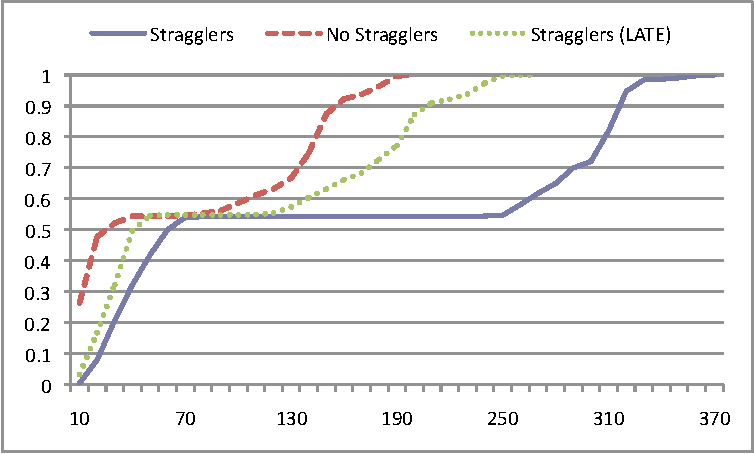
\includegraphics[width=0.95\linewidth]{graphs/reduce_stragglers}
  \caption{CDF of reduce task duration (secs), with and without stragglers.}
  \label{fig:ec2reduce}
  \vspace{-8pt}
\end{figure}

\subsection{Discussion}
The initial version of \BOOM-MR required one person-month of
development time. We spent an additional two person-months debugging
and tuning \BOOM-MR's performance for large jobs. \BOOM-MR consists of
55 Overlog rules in 396 lines of code, and 1269 lines of Java.
\BOOM-MR is based on Hadoop version 18.1; we estimate that we removed
6,573 lines from Hadoop (out of 88,864). The removed code contained
the core scheduling logic and the data structures that represent the
components listed in Table~\ref{tbl:hcatalog}. The Overlog patch that
replaces the original Hadoop scheduler contains an order of magnitude
fewer lines of code.  The performance of \BOOM-MR is very similar to
that of Hadoop MapReduce, as we discuss in Section~\ref{sec:eval}.

%% Our experience gutting Hadoop and inserting \BOOMA was not always
%% pleasant.  Given that we were committed to preserving the client API,
%% we did not take a ``purist'' approach and try to convert everything
%% into tables and Overlog rules.  For example, we chose not to
%% ``tableize'' the JobConf object, but instead to carry it through
%% Overlog tuples.  In our Overlog rules, we pass the JobConf object into
%% a custom Java table function that manufactures {\em task} tuples for
%% the job, subject to the specifications in the JobConf.

For this ``porting'' exercise, it was handy to leverage \JOL's Java interfaces
and draw the Java/Overlog boundaries flexibly.  This allowed us to focus on
porting the more interesting Hadoop logic into Overlog, while avoiding ports of
relatively mechanical details.  For example, we chose to leave the data
representation of the \emph{jobConf} as a Java object rather than flatten it
into a relation because it had no effect on the scheduling logic.

We found that scheduling policies were a good fit for a declarative language
like Overlog. In retrospect, this is because scheduling can be decomposed into
two tasks: \emph{monitoring} the state of a system and applying \emph{policies}
for how to react to changes to that state. Monitoring is well-handled by
Overlog: we found that the statistics about {\TT} state required by the LATE
policy are naturally realized as aggregate functions, and \JOL took care of
automatically updating those statistics as new messages from {\TT}s arrived. It
is also unsurprisingly that a logic language should be well-suited to specifying
policy. Overall, we found the \BOOM-MR scheduler much simpler to extend and
modify than the original Hadoop Java code, as demonstrated by our experience
with LATE\@.  Informally, the Overlog code in \BOOM-MR seems about as complex as
it should be: Hadoop's MapReduce task coordination logic is a simple and clean
design, and the compactness of \BOOM-MR reflects that simplicity appropriately.
